% ---
% Capitulo de revisão de literatura
% ---


\chapter{Trabalhos Relacionados}\label{referencial_teorico}
Aqui será dedicado a descrever os trabalhos relacionados ao tema desta pesquisa.

O trabalho \cite{kalambet2011noise} descreve um método de filtragem de ruido baseado em intervalo de confiança, com uma abordagem que utiliza matrizes para evitar dados discrepantes deixando-os como estão, o estudo enfatiza alguns dos problemas encontrados nos filtros mais utilizados, como a falta de critério claro da filtragem e interferência no resultado final. A pesquisa \cite{madhale2020adaptive} apresenta uma técnica de remoção de ruido adaptável baseada em intervalo de confiança adaptável e orientado a dados, para limpeza de valores do monitoramento através de eletroencefalograma que analisa a atividade elétrica cerebral espontânea, o trabalho obteve sucesso reduzindo significadamente as taxas de ruido tornando a dinâmica do cérebro mais analisável no exame e com menos ruido.

% O autor \cite{International_Conference__Zhuang} \cite{particle_swarm__Narkhede}\cite{Statistical_approach__Elnahrawy}


% O autor \cite{Garcia} define uma serie de estrategias 
% para avaliar um RTOS moderno, passando por diversos pontos importantes em um sistema de tempo real, 
% como resposta a eventos externos, compartilhamento de recurso e sincronização entre tarefas. 
% Em \cite{Raymundo} o autor se baseia nestas estrategias, 
% implementando com novas tecnicas em 5 sistemas operacionais diferentes, inclusive nos dois 
% sistemas propostos aqui neste trabalho, seu trabalho tem um foque em internet das coisas, 
% tendo como base a plataforma de hardware NXP/Freescale FRDM-K64F.
% No estudo \cite{nicolas2019avaliaccao}, o autor busca compreender e avaliar o funcionamento 
% do FreeRTOS embarcado em um cubesat real, o estudo explica o funcionamento do sistema em 
% cada um de seus pontos como, controle e escalonamento de tarefas, gerenciamento de filas e 
% memória, erros comuns e etc. Para avaliar o sistema, o mesmo foca numa serie de experimentos 
% que são voltados ao funcionamento do sistema em um ambiente real de operação, tendo como vista 
% problemas relacionados a radiação, perca de memória, corrompimento de dados e estouro de memória.
% Os trabalhos trabalhos de \cite{Garcia} e \cite{Raymundo} tem foque nas qualidades do sistema, já 
% o trabalho de \cite{nicolas2019avaliaccao} foca no desempenho do sistema em ambiente real, perante 
% a problemas externos e de missão.


\chapter{Revisão Bibliométrica sobre Filtragem de dados de sensores}\label{referencial_teorico}

Nesta seção são consideraras as informações referentes á produção acadêmica mundial, que abordam os termos em ingles Noise reduction, noise abatement, Filtering algorithm e Sensor, significando em sequencia redução de ruído, algoritmos de filtragem e sensores. 

Ambos os tópicos foram pesquisados na base IEEE Xplore, com a busca limitada aos termos noise reduction e noise abatement no titulo do documento e filtering algorithm, sensor e noise reduction apenas no texto completo, delimitando exclusivamente aos artigos de 2018 a 2022. Resultando em 675 resultados sendo eles 450 conferencias, 215 artigos, 8 artigos com acesso  antecipado e 2 revistas, foi realizado uma revisão bibliométrica sobre estes 215 artigos resultantes. 

Dados provenientes de sensores são constantemente bombardeados com interferências aleatórias do ambiente onde se encontram, também devido a baixa qualidade provenientes dos sensores de baixo custo disponíveis, inserindo valores incorretos que são caracterizados como ruídos nas amostras. Esse problema desperta um grande interesse de pesquisadores, que buscam lidar com o tratamento e a filtragem de dados ruidosos provindos de sensores diversos, o artigo \cite{chiang_noise_reduction_in_ECG} se destaca por ser o trabalho mais citado nessa pesquisa bibliométrica, o mesmo aborda o problema da interferência de ruídos nos sinais provindos dos sensores de eletrocardiograma, esses dados podem ser contaminados por fatores como a estática da pele ou mesmo pela respiração do paciente, para isso técnicas como wavelet são muito populares, utilizadas para filtrar dados cancelando o ruído analisando mudanças bruscas ou picos na frequência do sinal, o método de decomposição do modo empírico também e bastante utilizado, definindo fronteiras entre o local máximo e mínimo de uma subtração de sequencia que consequentemente ajudam na triagem do tratamento do sinal.   

\begin{figure}[H]
	\centering
	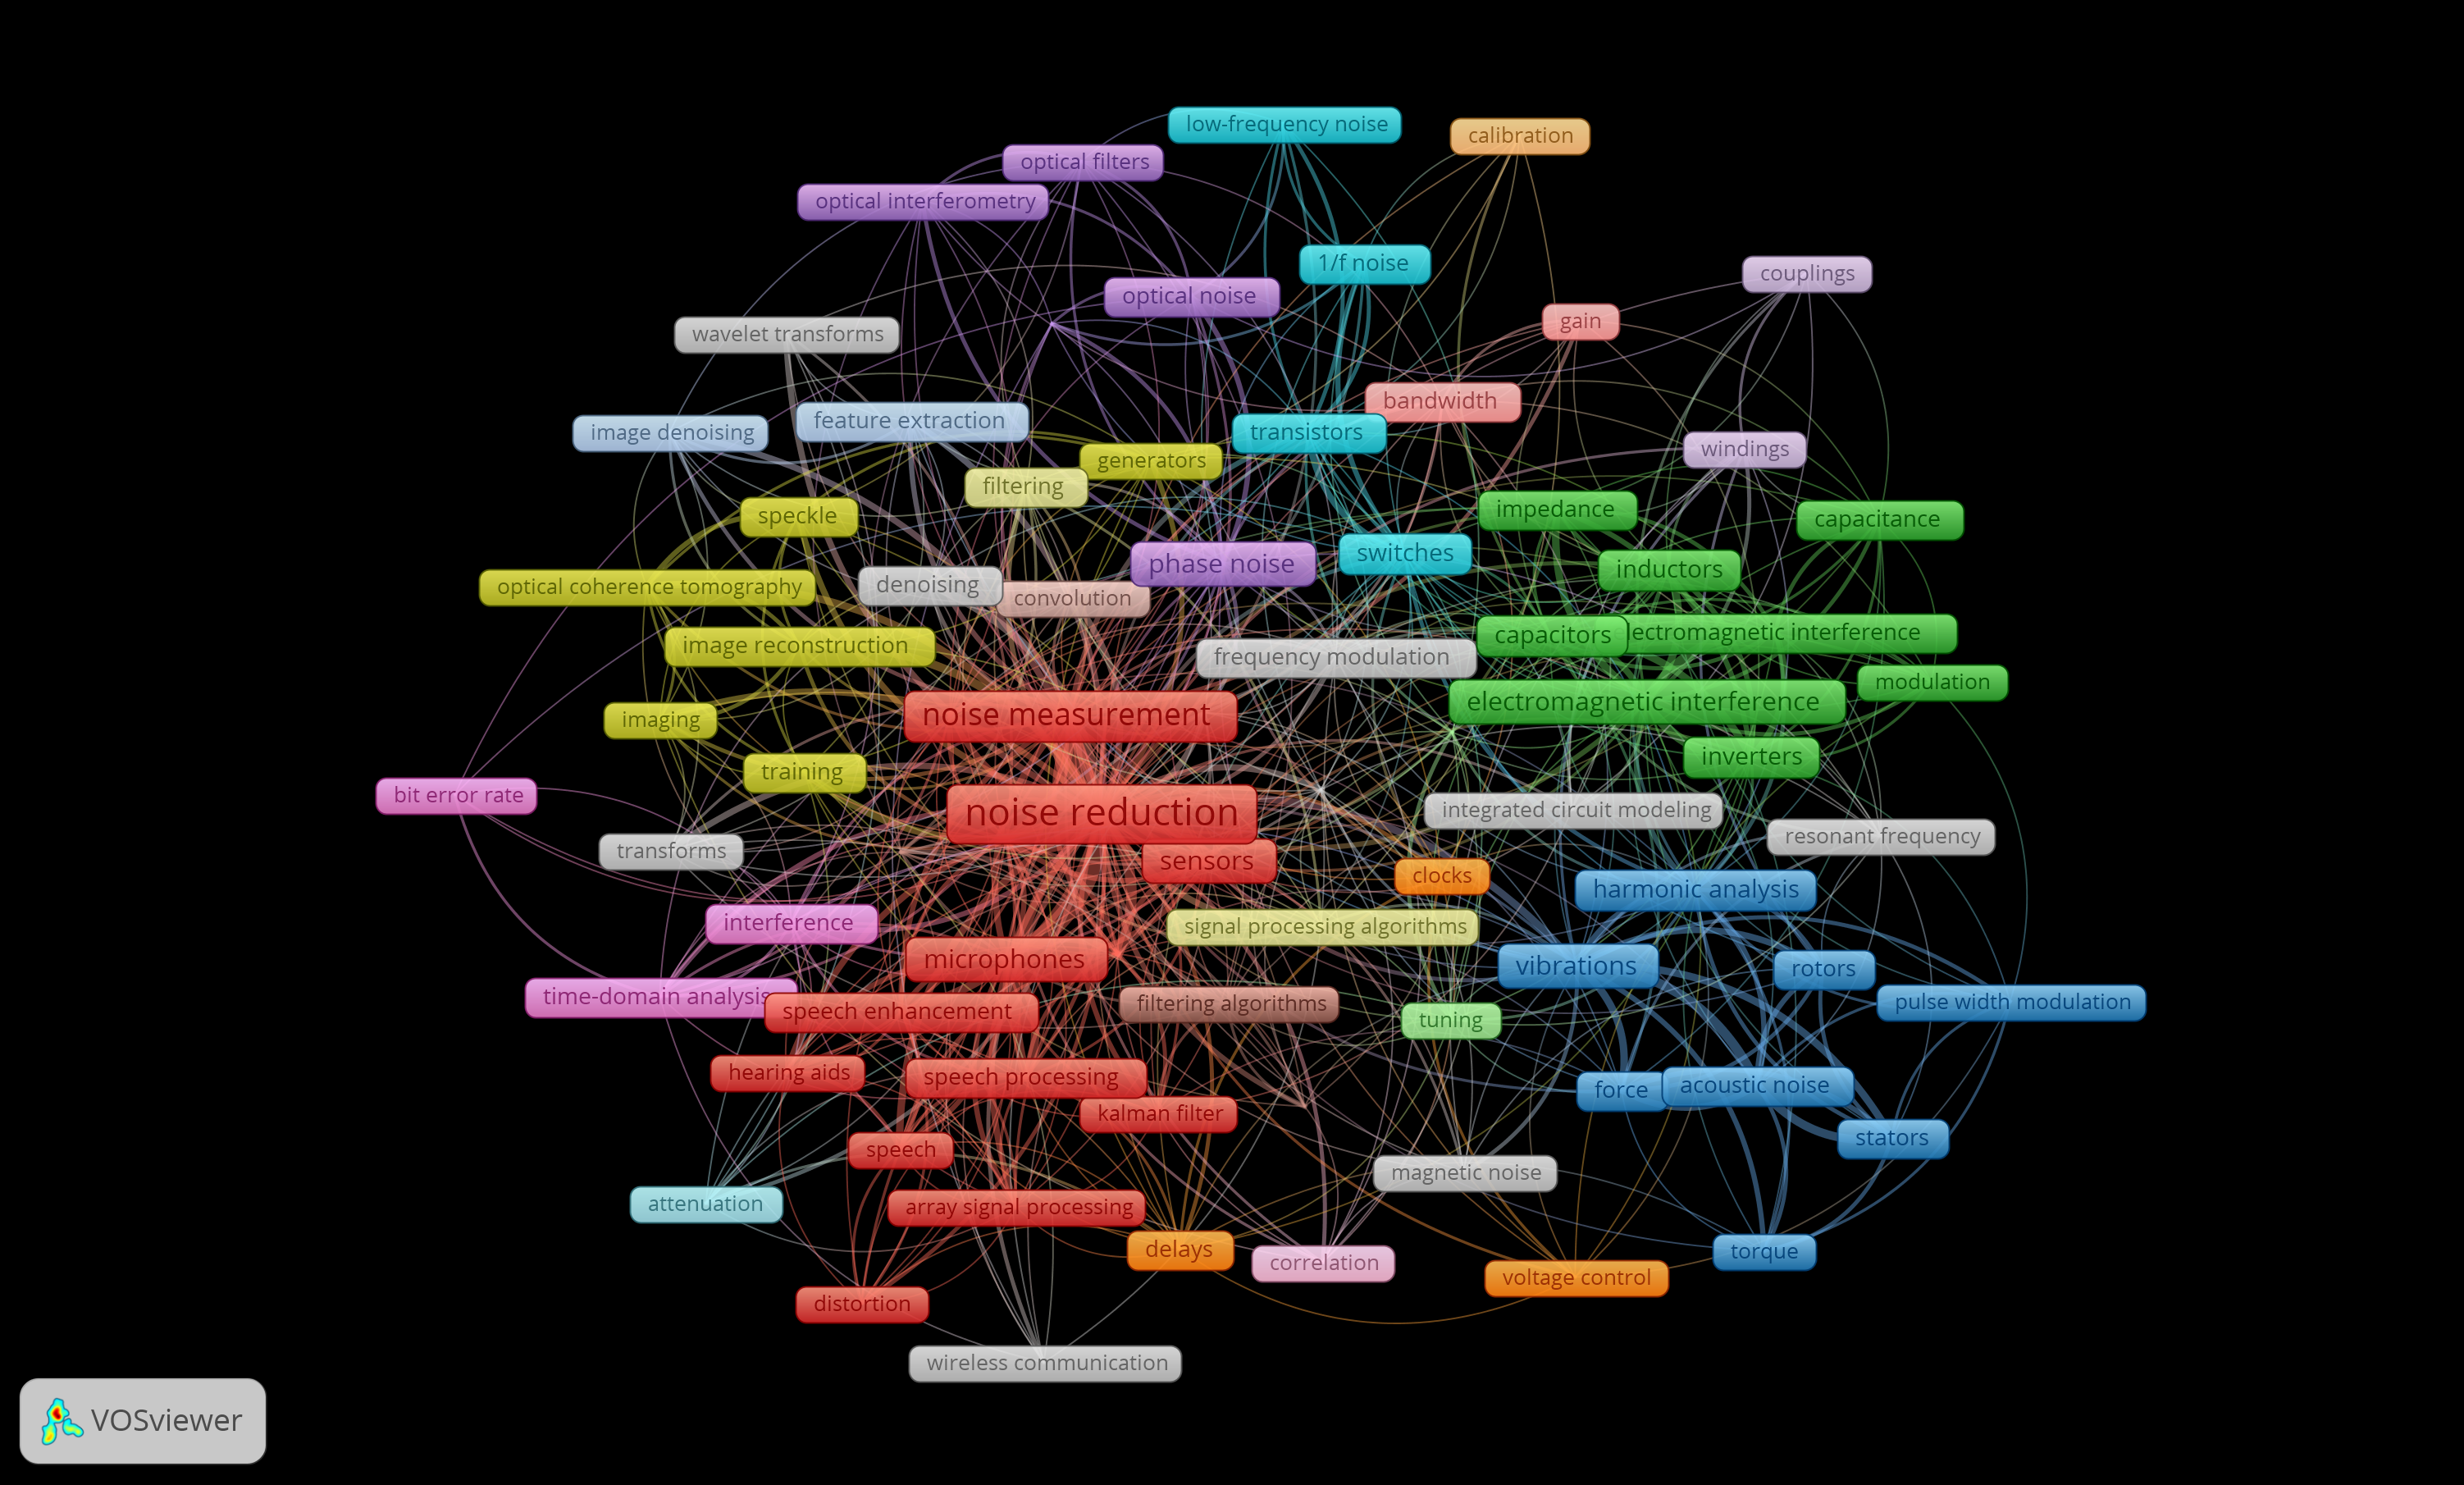
\includegraphics[width=15cm]{anexos/ris/IEEE/Noise_reduction_and_noise_abatement_andsensor_filtering_algorithm/network_visualization_with_lines.png}
	\caption{Mapa de visualização de rede}
	Fonte: Autor com base no Software VOSViwer.
	\label{fig: network_visualization_with_lines}
\end{figure}

A Figura~\ref{fig: network_visualization_with_lines} representa um mapa de visualização de rede, onde podemos visualizar os termos mais predominantes. Aqui são percebidos o termos que se repetiram mais de 5 vezes nos textos e resumos, nota-se a formação de grupos de acordo com suas áreas de atuação, alguns termos em destaque são em azul relacionados a motores, vibrações e forças mecânicas, os em verdes referentes a componentes eletrônicos, roxo a sensores ópticos, amarelo o tratamento de imagem e em vermelho sensores embarcados e processamento de sinais. 


Todos essas expressões aprofundam a problemática no qual tratamento de ruídos, algoritmos de filtragem e sensores estão correlacionados, indo de problemas em programas de computador a desenvolvimento de circuitos eletrônicos e peças mecânicas. O error na fabricação de sensores ópticos pode levar a fenômenos de interferência nos resultados \cite{liu_interference_stripe}, essas anomalias prejudicam sistemas de medição holográfica digital, afim de melhorar a captação de imagens sem ruído o autor propõem um novo método de processamento de imagem utilizando pirâmide laplaciana para destacar o ruído de faixa de interferência.


\begin{figure}[H]
	\centering
	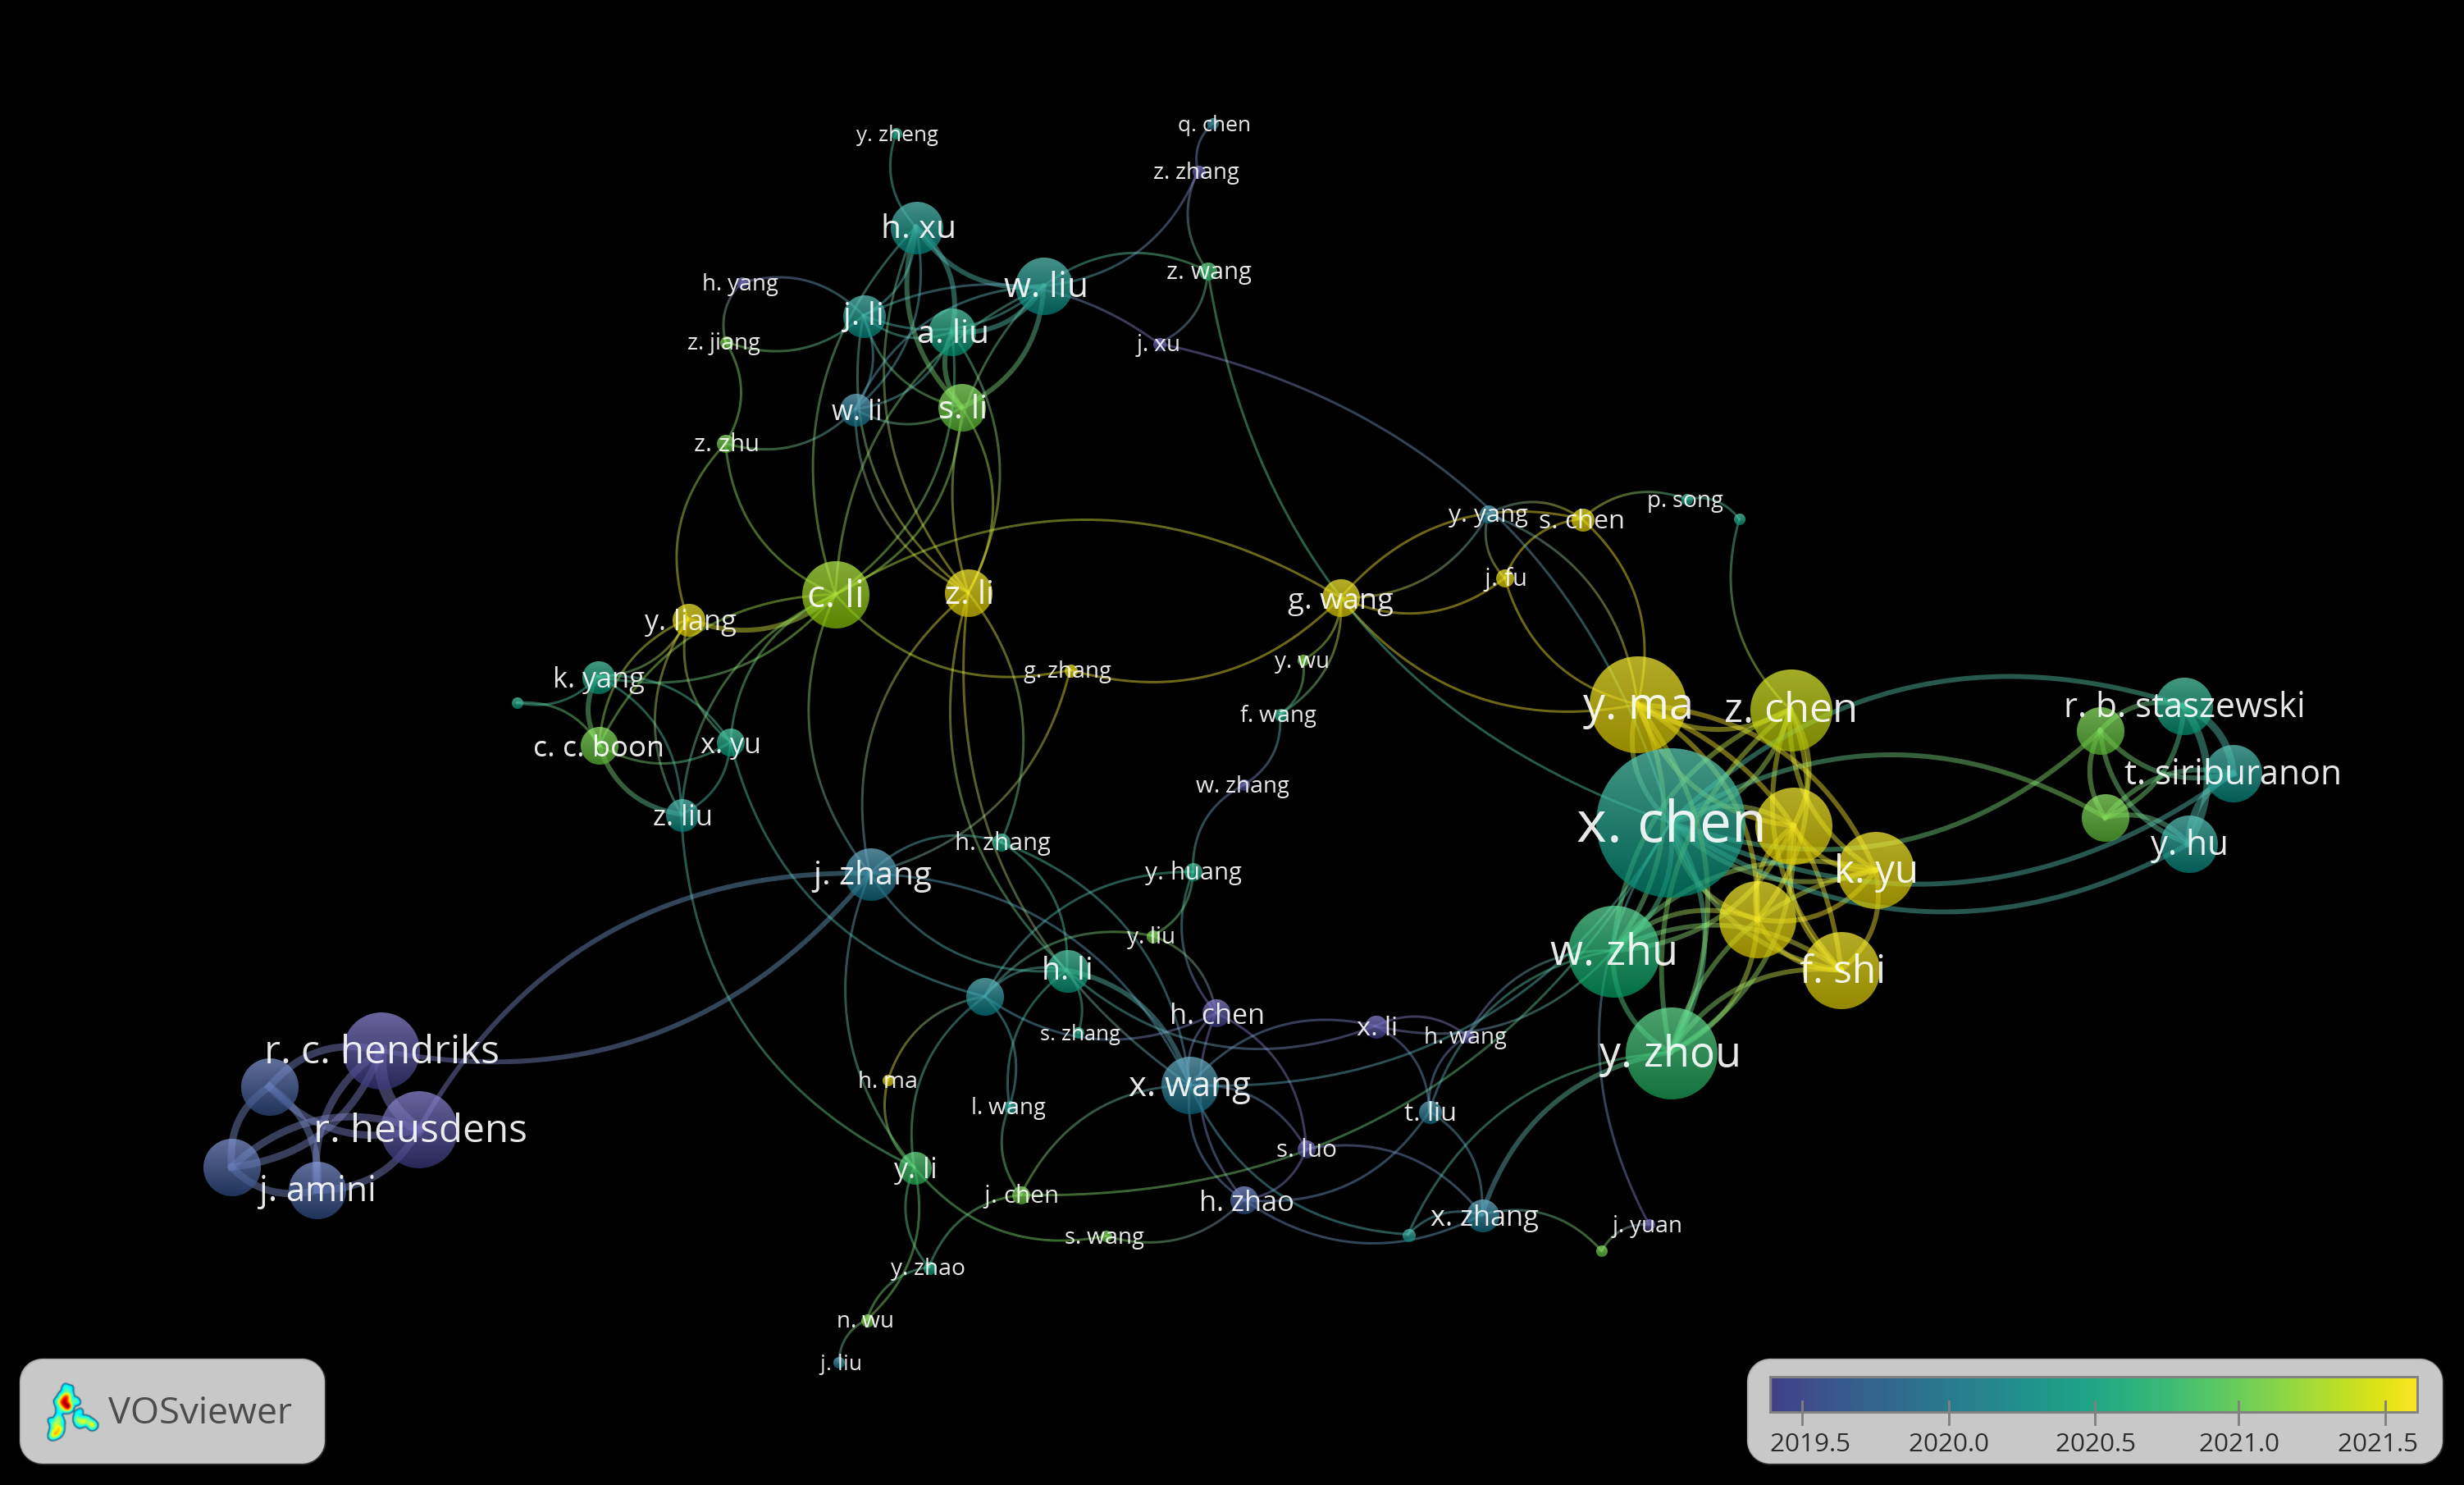
\includegraphics[width=15cm]{anexos/ris/IEEE/Noise_reduction_and_noise_abatement_andsensor_filtering_algorithm/overlay_visualization_cites.png}
	\caption{Mapa de visualização autores}
	Fonte: Autor com base no Software VOSViwer.
	\label{fig: overlay_visualization_cites}
\end{figure}

A Figura~\ref{fig: overlay_visualization_cites} apresenta um mapa semelhante a figura anterior, a imagem destaca os autores mais citados em média, destacando-os pelo tamanho do circulo atrás de seu nome, e pela sua presença em artigos mais recentes de acordo com a cor mais amarelada. 
Em \cite{duarte_speckle_noise} afim de melhorar aplicações biomédicas em imagens de ultrassom, o trabalho descreveu 27 técnicas para tratamento eliminação de ruido em em imagens de ultra-som, essas imagens são de verdadeira importância para o diagnóstico clínico e procedimentos terapêuticos não invasivos, fundamentais em diversas áreas da saúde.

Na Figura~\ref{fig: overlay_visualization} abaixo visualiza-se um mapa de sobreposição, onde os vocabulários mais amarelos representam os que se encontram em publicações em media mais recentes, também podemos notar a relação entre as palavras encontradas em todos os títulos e resumos. 

\begin{figure}[H]
	\centering
	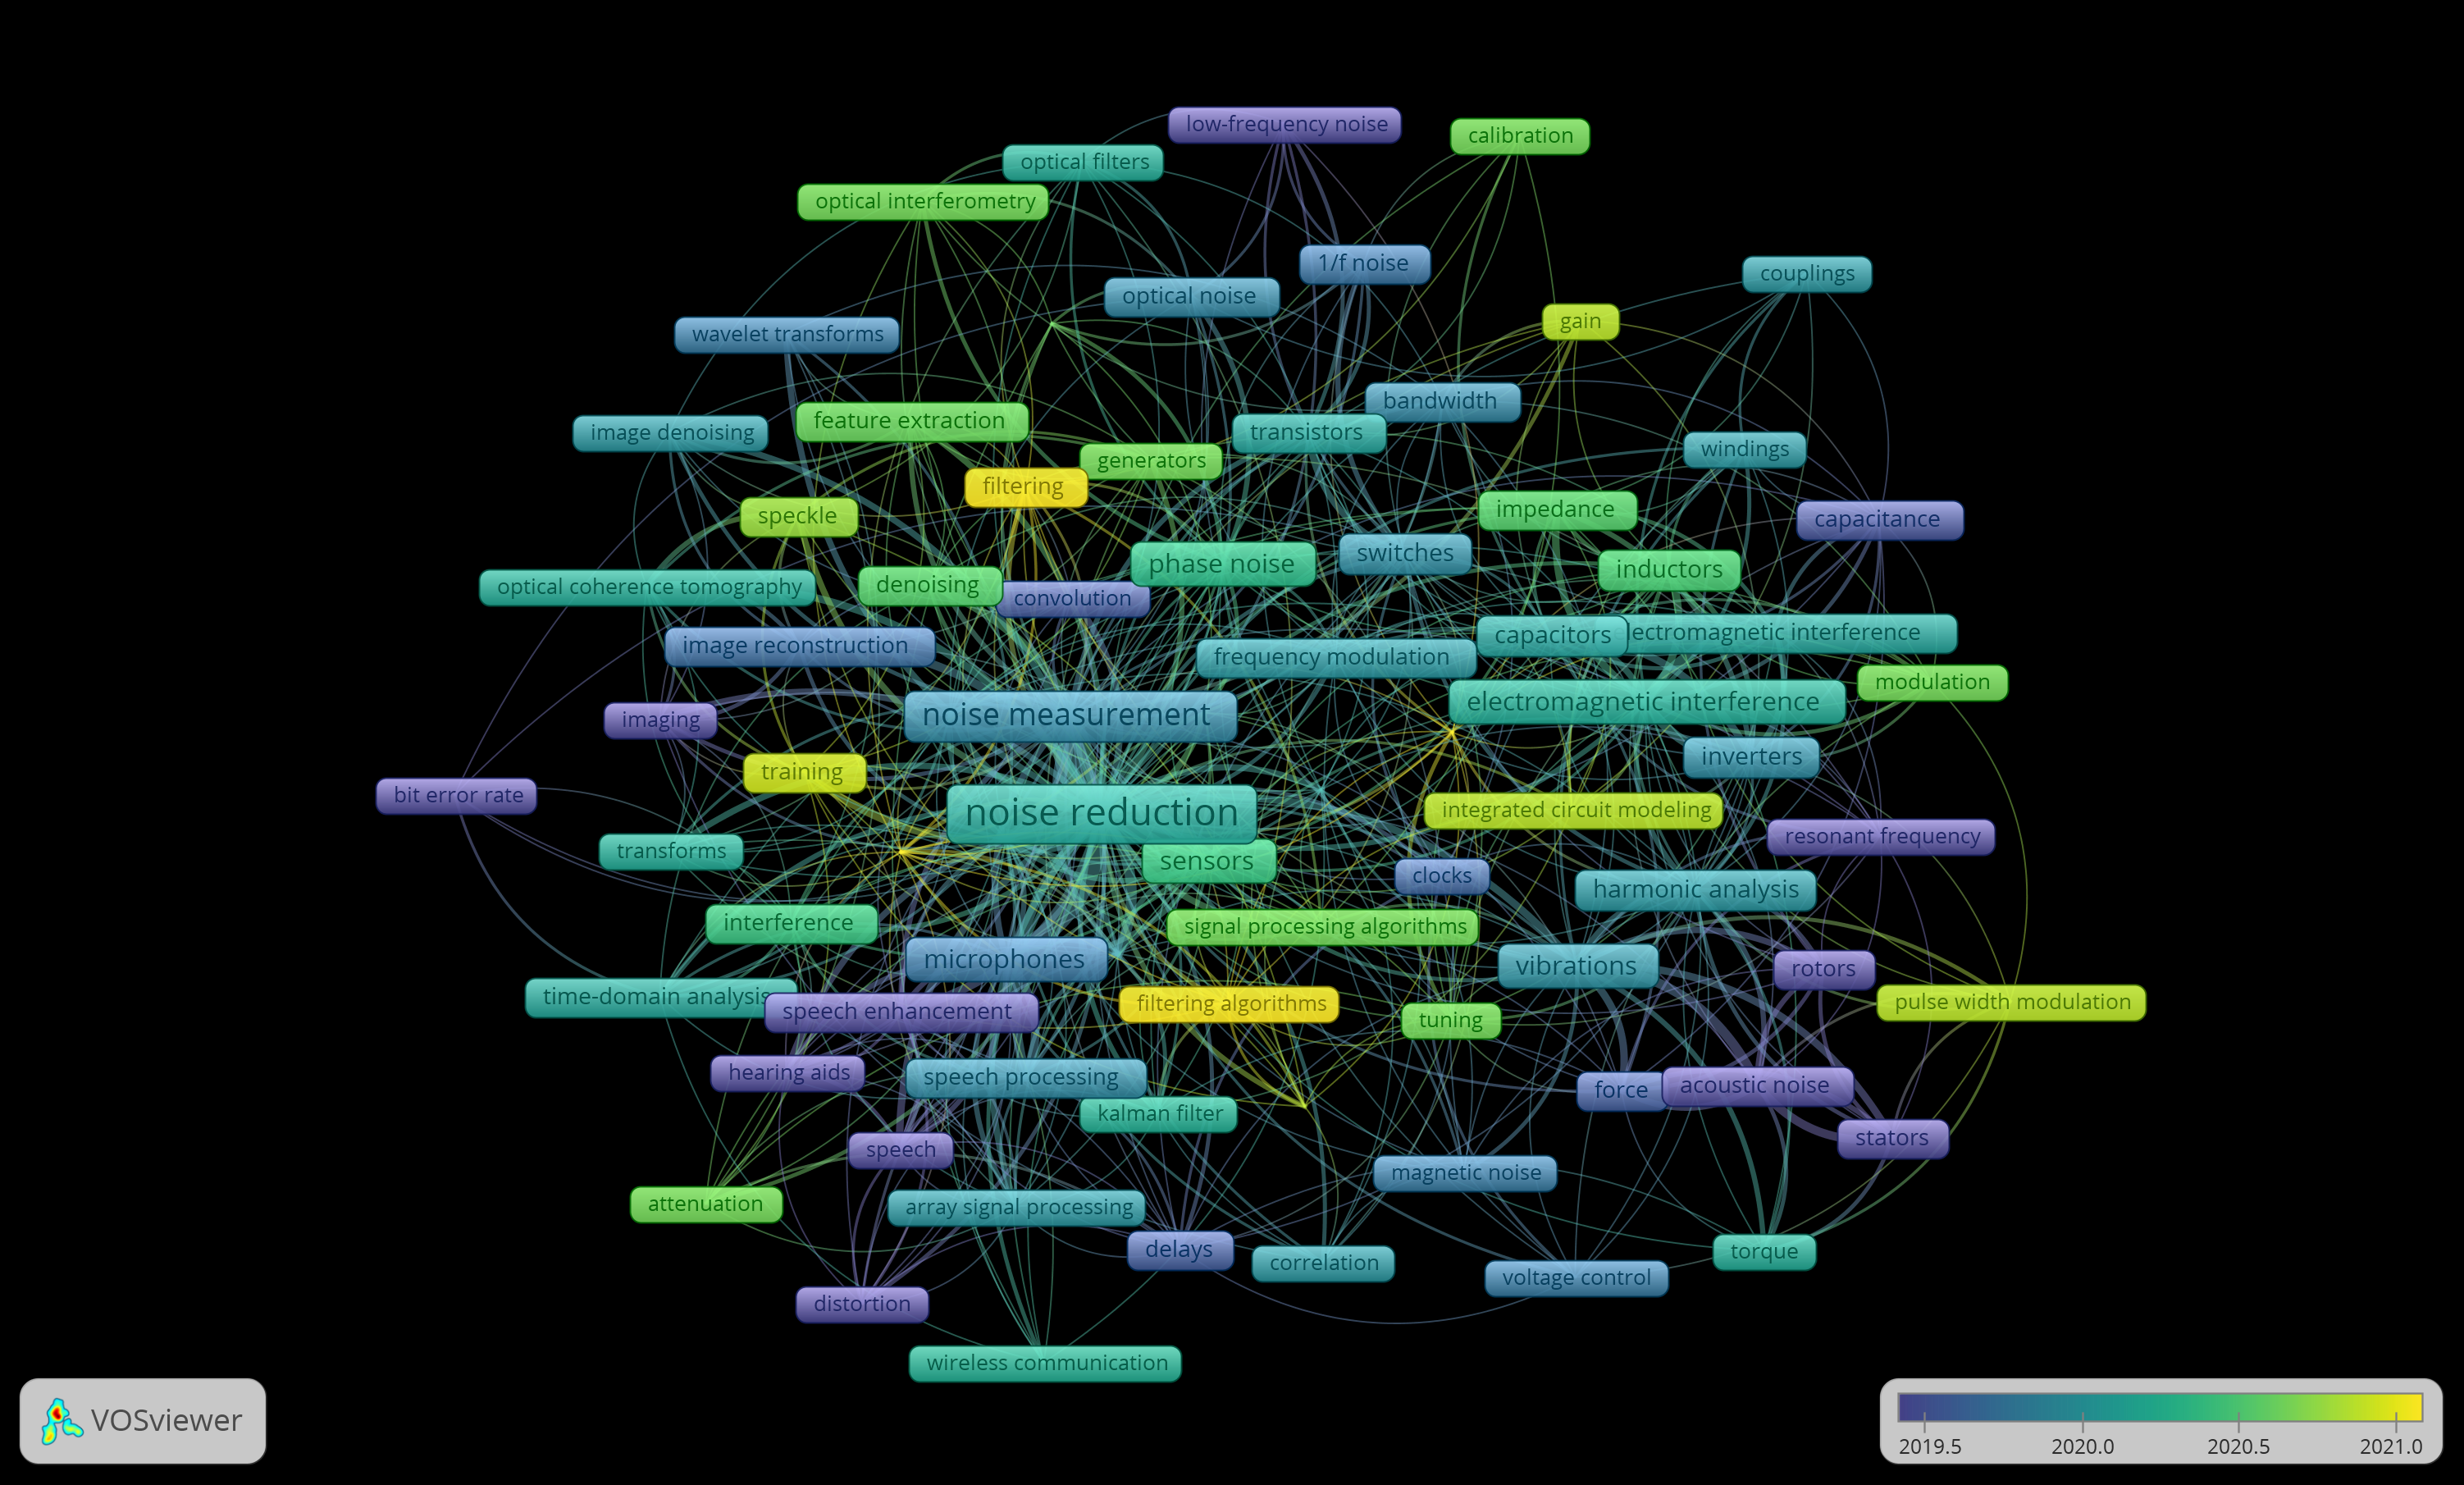
\includegraphics[width=15cm]{anexos/ris/IEEE/Noise_reduction_and_noise_abatement_andsensor_filtering_algorithm/overlay_visualization.png}
	\caption{Mapa de sobreposição}
	Fonte: Autor com base no Software VOSViwer.
	\label{fig: overlay_visualization}
\end{figure}

Há de se notar que os termos filtragem e algoritmos de filtragem se destacam pela sua quantidade acima da media de trabalhos mais recentes, não se distanciando das definições de redução de ruído, sensores e algoritmos de processamento de sinais próximos do centro do mapa.

% \subsection{Zephyr RTOS}
% Há mais de 20 anos nascia o primeiro RTOS do mercado, desde então outros sistemas tem trazido 
% contribuições para o mundo embarcado. Um sistema operacional de tempo real se difere de um sistema 
% operacional comum por depender diretamente do momento em que a ação foi produzida, buscando 
% manter o tempo de mudança de contexto mínimo e gerenciando a execução de tarefas de acordo com 
% suas prioridades \cite{Hambarde}. Os aplicativos de tempo real se tornaram populares devido a 
% complexidade dos sistemas modernos, paralelo a isso o mercado de RTOS é bastante grande, com 
% diversos antagonistas fornecendo ferramentas para resolver problemas de tempo real em diversas 
% plataformas e de diversas maneiras, tornando a escolha cada vez mais difícil \cite{Hambarde}.


% Zephyr é um RTOS de código aberto gerido pela Linux Foundation, construído sobre recursos
% limitados e pensado em segurança e proteção, frequentemente adotado em sistemas críticos \cite{Zhao}.
% Suportando uma grande variedade de placas de hardware e utilizado por empresas como Google, Intel
% e Facebook. Oferece cooperatividade e segmentação preemptiva, alocação estática de memória,
% isolamento de thread e dispositivos de proteção de memória \cite{nyffenegger2020connecting}.

% \begin{figure}[H]
% 	\centering
% 	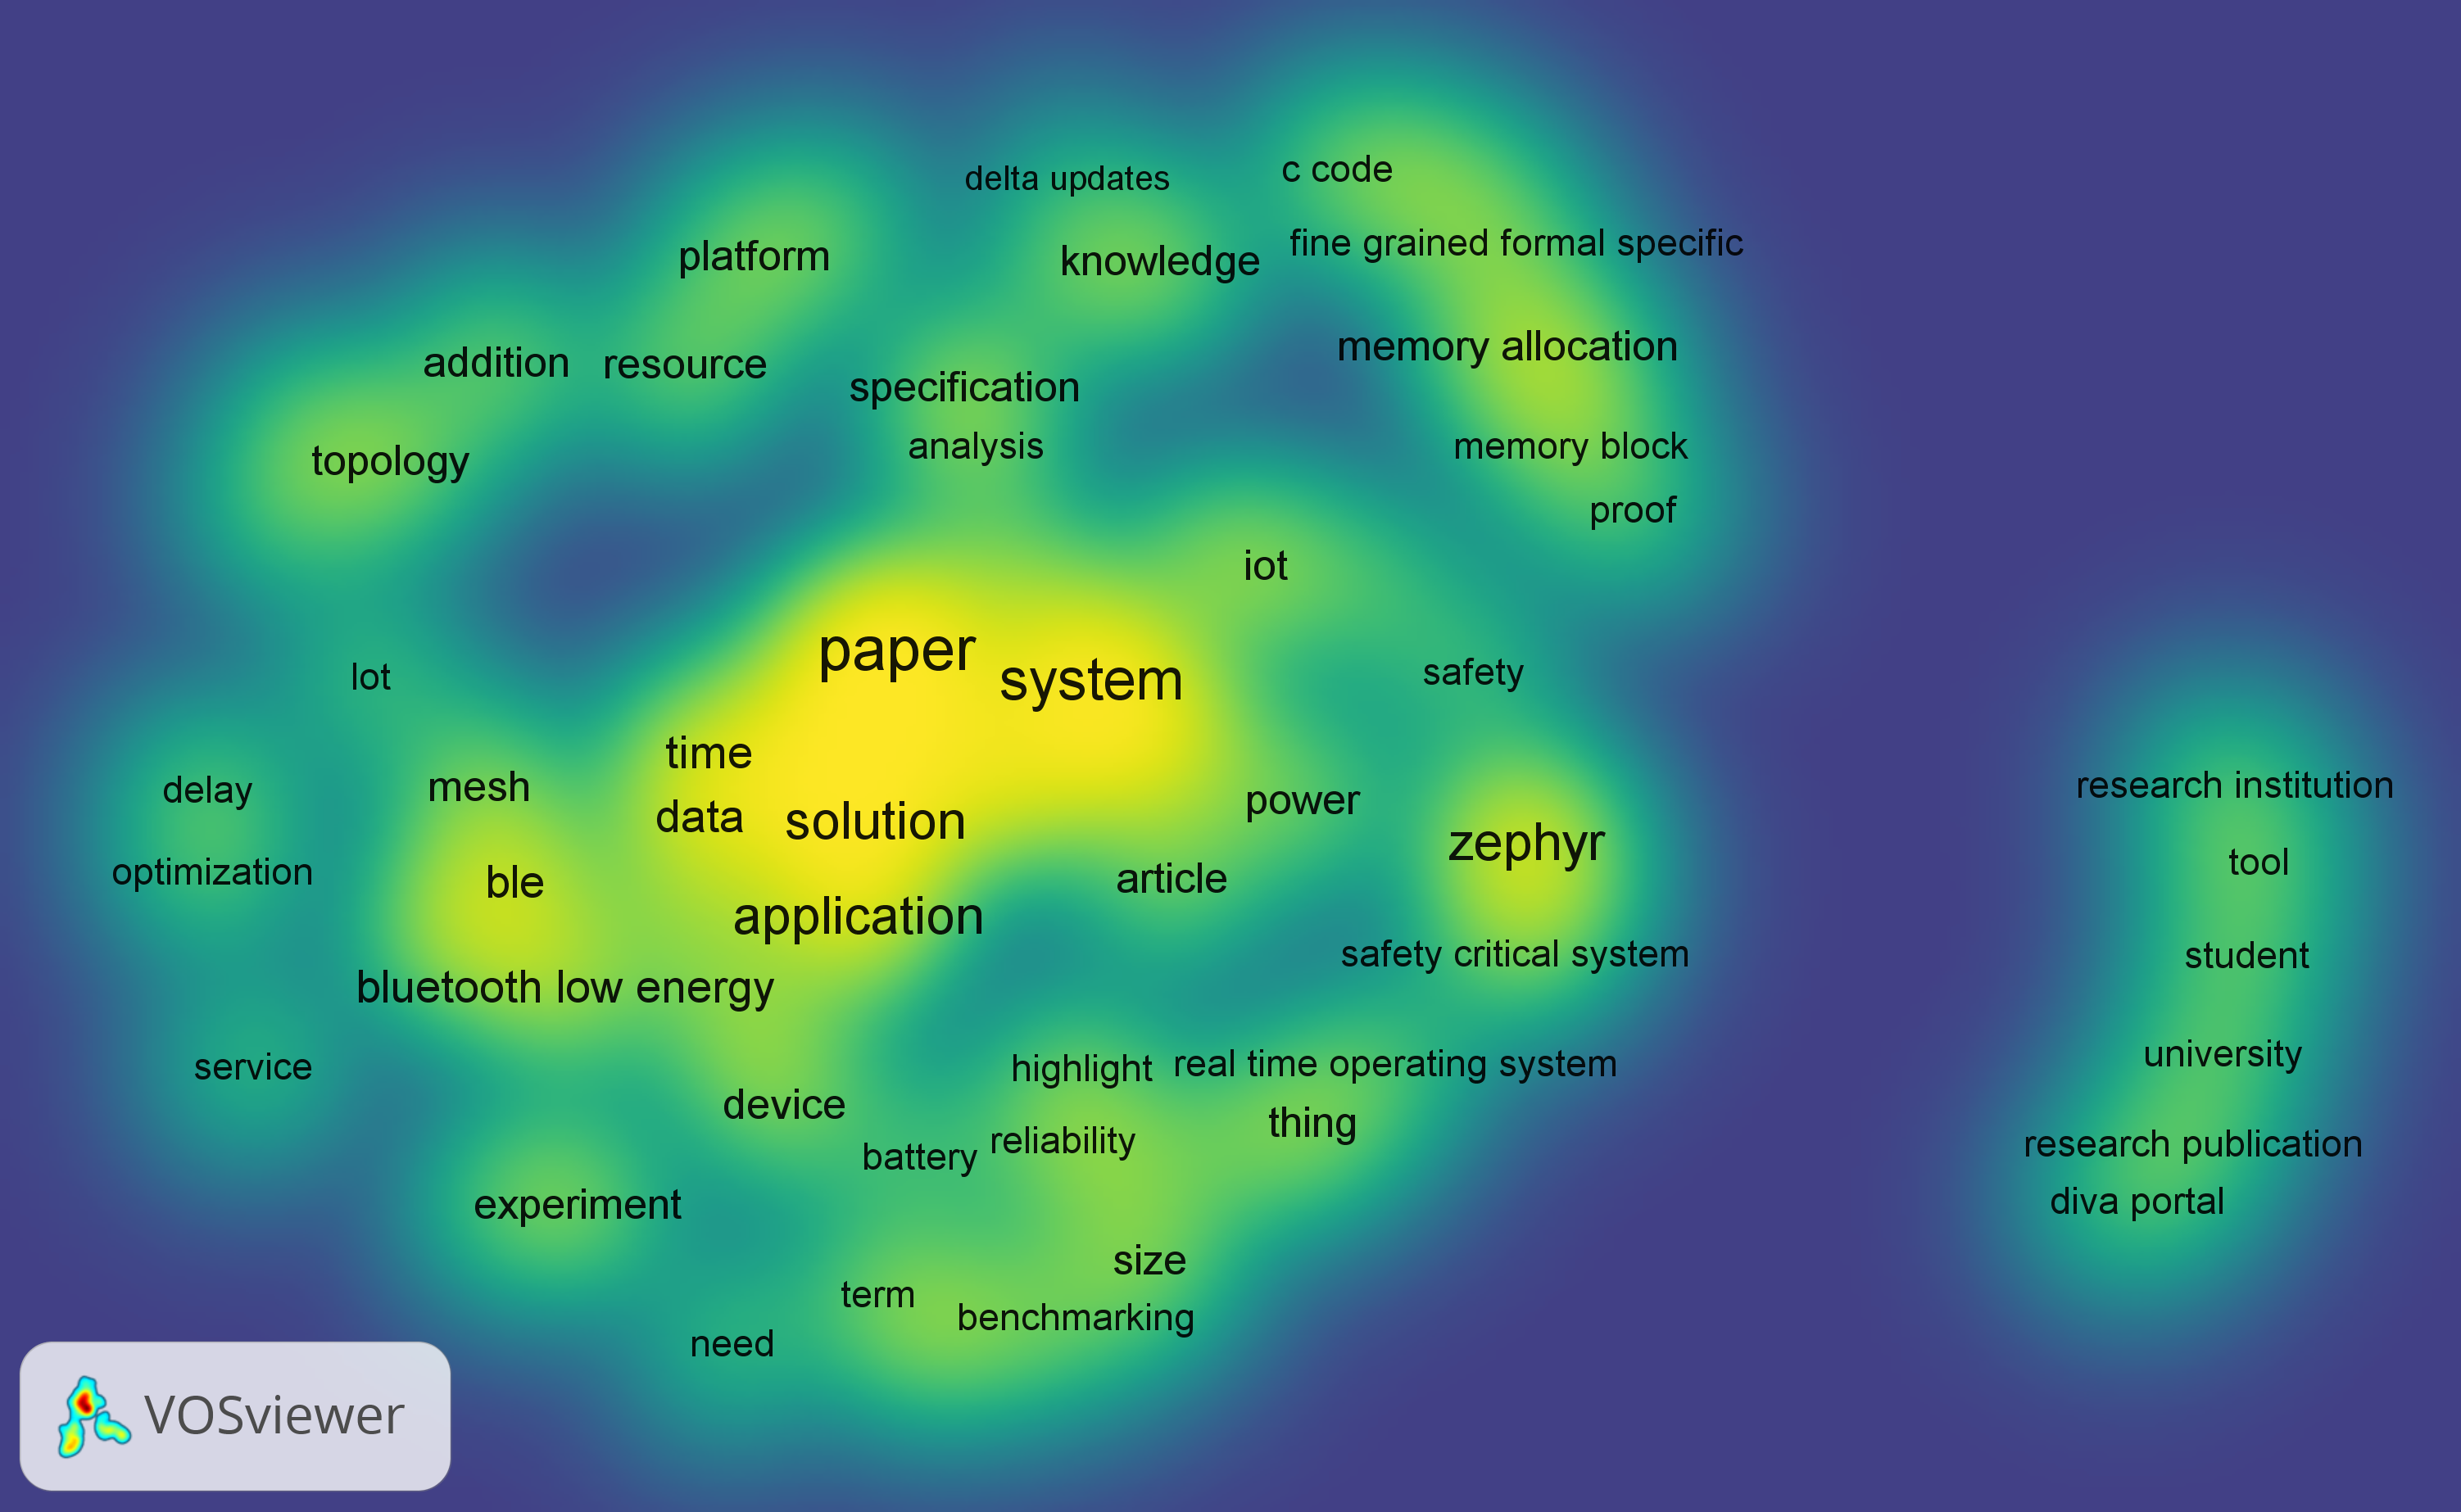
\includegraphics[width=15cm]{imagens/Zephyr_RTOS_Density_Visualization.png}
% 	\caption{Mapa de visualização de densidade sobre o termo "Zephyr RTOS"}
% 	Fonte: Autor com base no Software VOSViwer.
% 	\label{fig: Zephyr Density Visualization}
% \end{figure}

% A Figura~\ref{fig: Zephyr Density Visualization} representa uma espécie de "mapa de calor" sobre o 
% tema "Zephyr RTOS" no mecanismo de busca Google Scholar, ao seu redor pode-se notar termos que 
% remetem a RTOS como "safety critical system", "iot", "bluetooth low energy" e "memory allocation". 
% Também e possível notar os termos "solution", "application", "service" e "plataform" que reforçam a 
% ideia de que zephyr é amplamente utilizada em diversas plataformas e projetos\cite{nyffenegger2020connecting}.

% \begin{figure}[H]
% 	\centering
% 	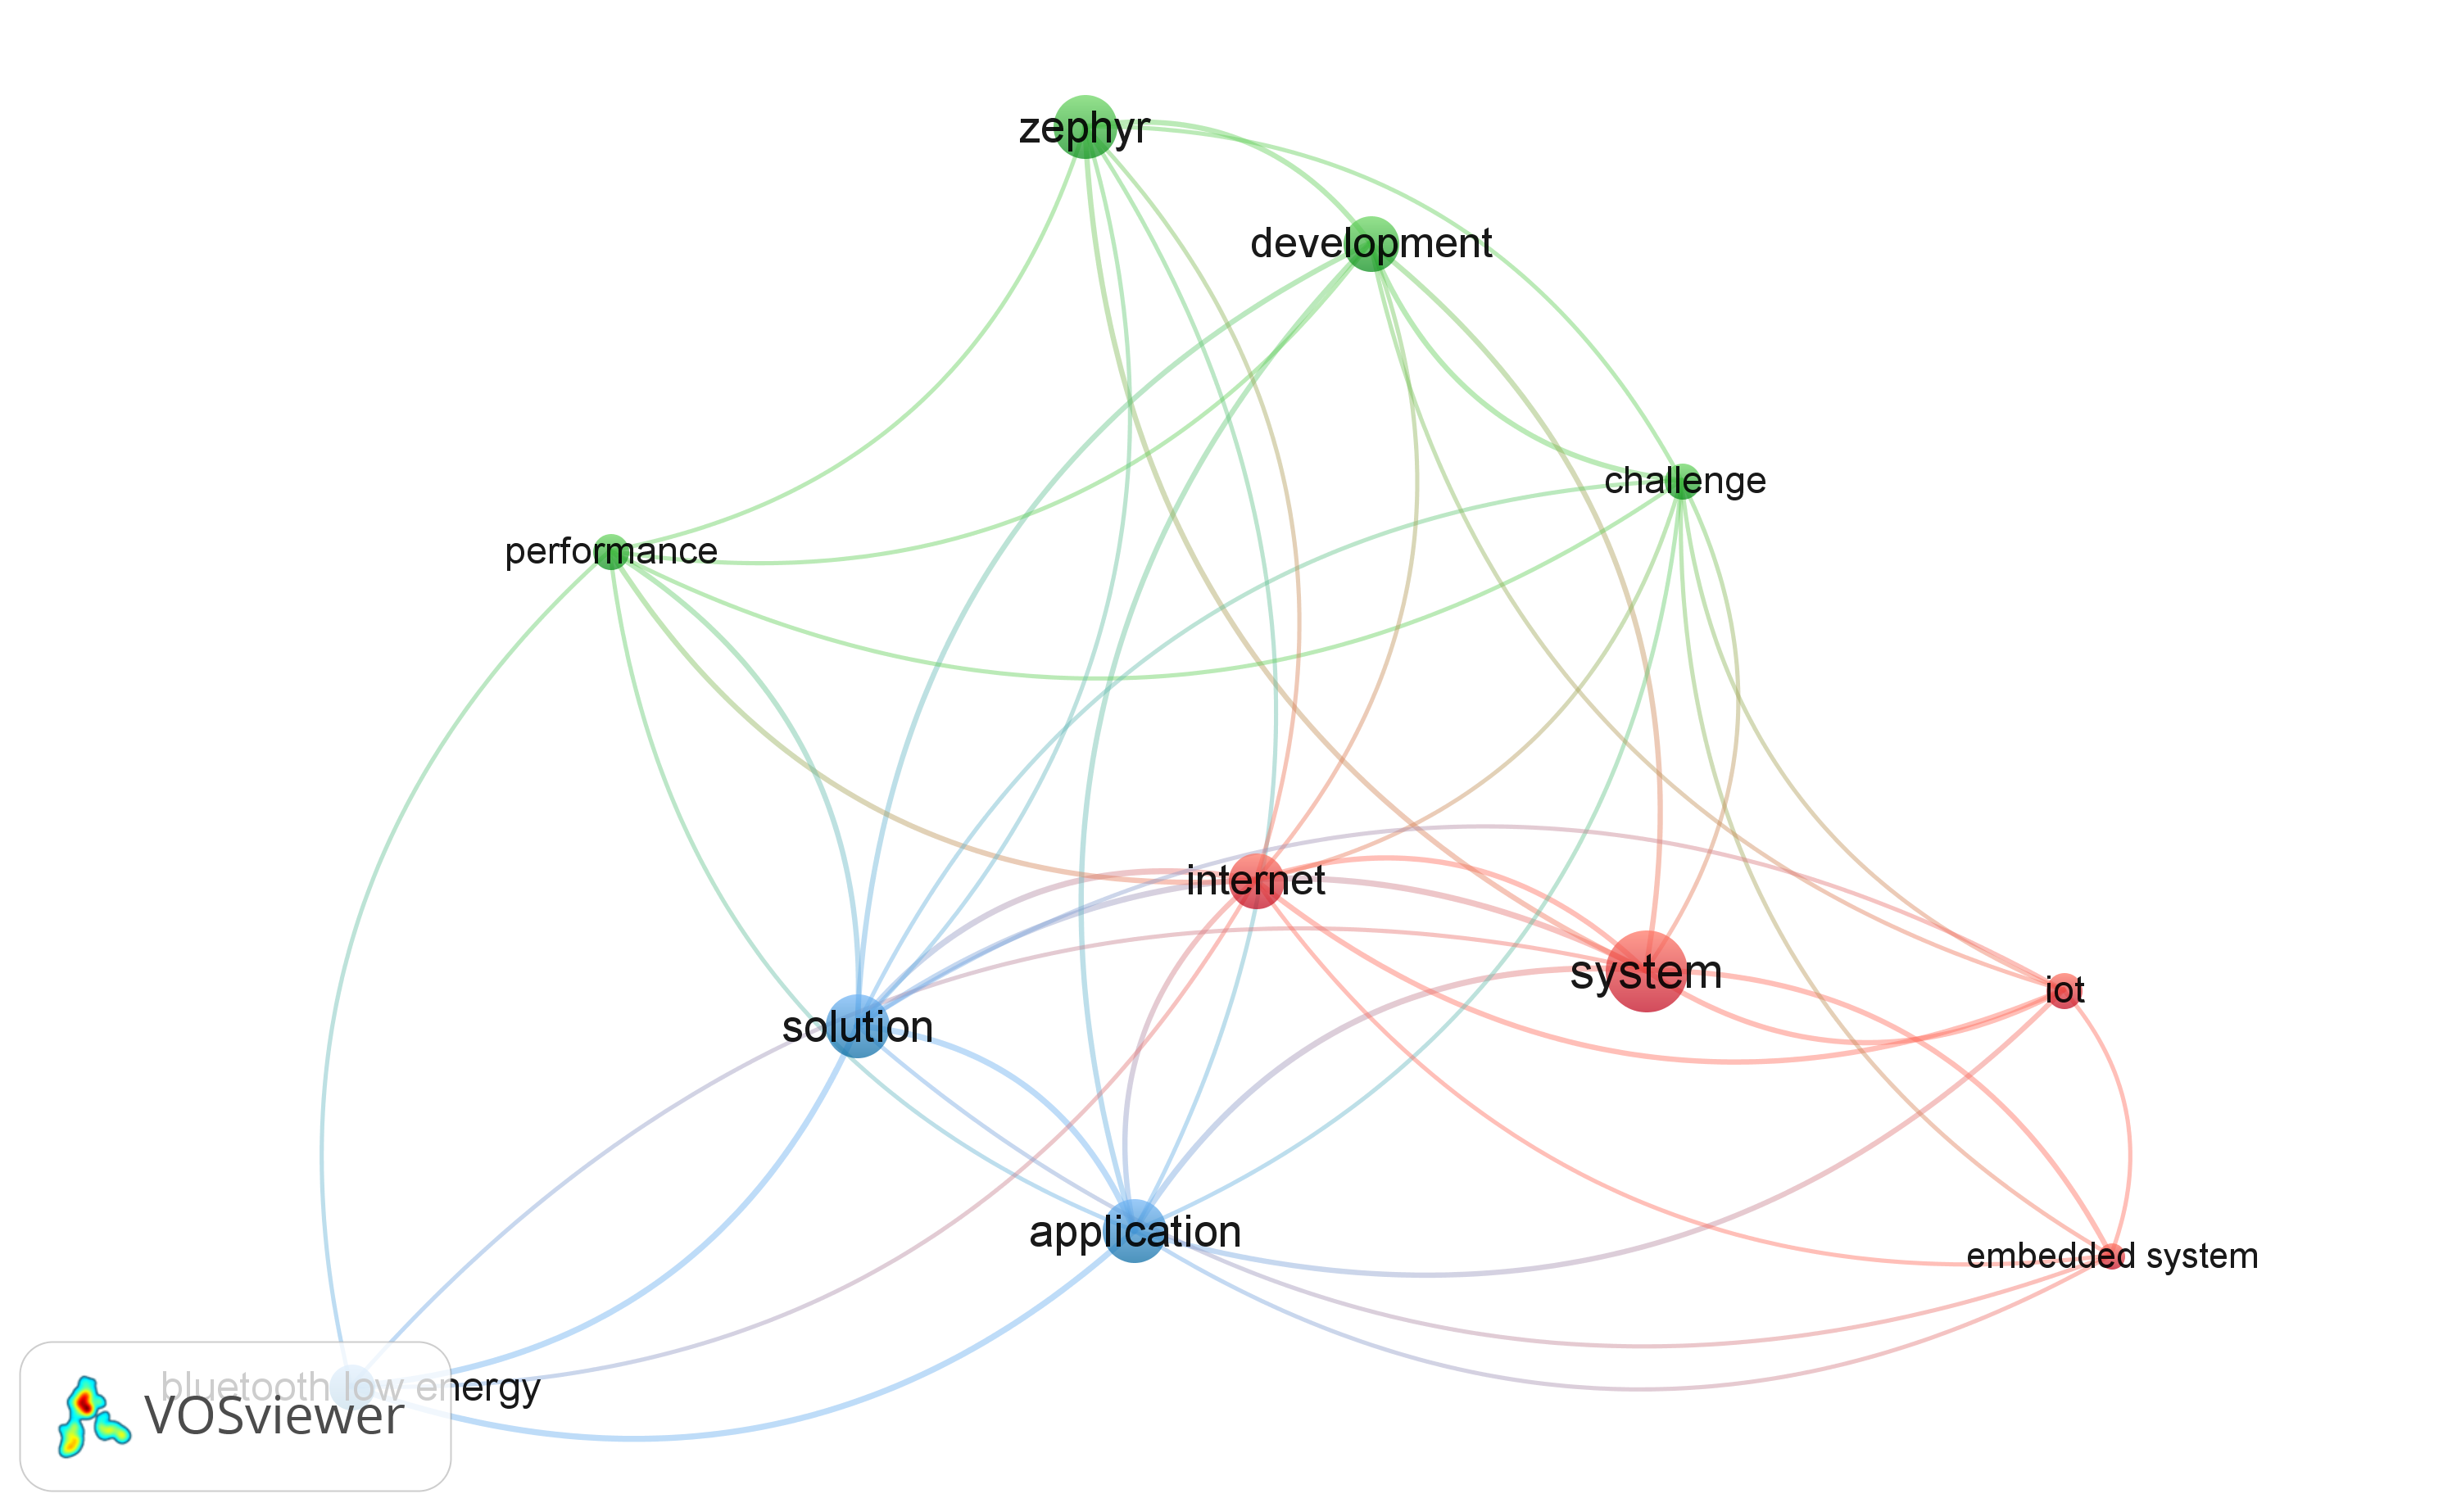
\includegraphics[width=15cm]{imagens/Zephyr_RTOS_Network_visualization.png}
% 	\caption{Mapa de visualização de rede sobre o termo "Zephyr RTOS"}
% 	Fonte: Autor com base no Software VOSViwer.
% 	\label{fig: Zephyr Network Visualization}
% \end{figure}

% A Figura~\ref{fig: Zephyr Network Visualization} demonstra uma rede de conexões entre o termo "Zephyr RTOS" 
% e outros termos populares em sua pesquisa, nota-se conexões importantes entre zephyr e termos importante sem 
% sua área. O tempo iot esta diretamente ligado a sistemas embarcados, sendo ligado ao zephyr através do termo 
% "internet", o sistema é construído e mantido por diferentes empresas que trabalham no campo IOT 
% \cite{huber_porting_2019}.


% \subsection{Software CubeSat}
% Para afunilar este estudo bibliométrico mais especifico para o termo central deste trabalho, realizou-se o 
% levantamento sobre os termos "Cubesat SO", na base de trabalhos e citações Google Acadêmico, foi selecionado 
% do período de 2012 a 2021 sendo encontrados aproximadamente 16.900 resultados, entre artigos, livros, 
% citações e outros materiais acadêmicos. CubeSats são pequenos satélites limitados a cubos de 10cm³ atualmente 
% muito populares, criado por Dr. Jordi Puig-Suari e Bob Twiggs, sendo uma espaçonave de custo e lançamento 
% relativamente acessível \cite{Manyak2011FaultTA}. Na Figura~\ref{fig: Cubesat Density Visualization}nota-se 
% os termos com mais destaques encontrados na busca feita neste trabalho.


% \begin{figure}[H]
% 	\centering
% 	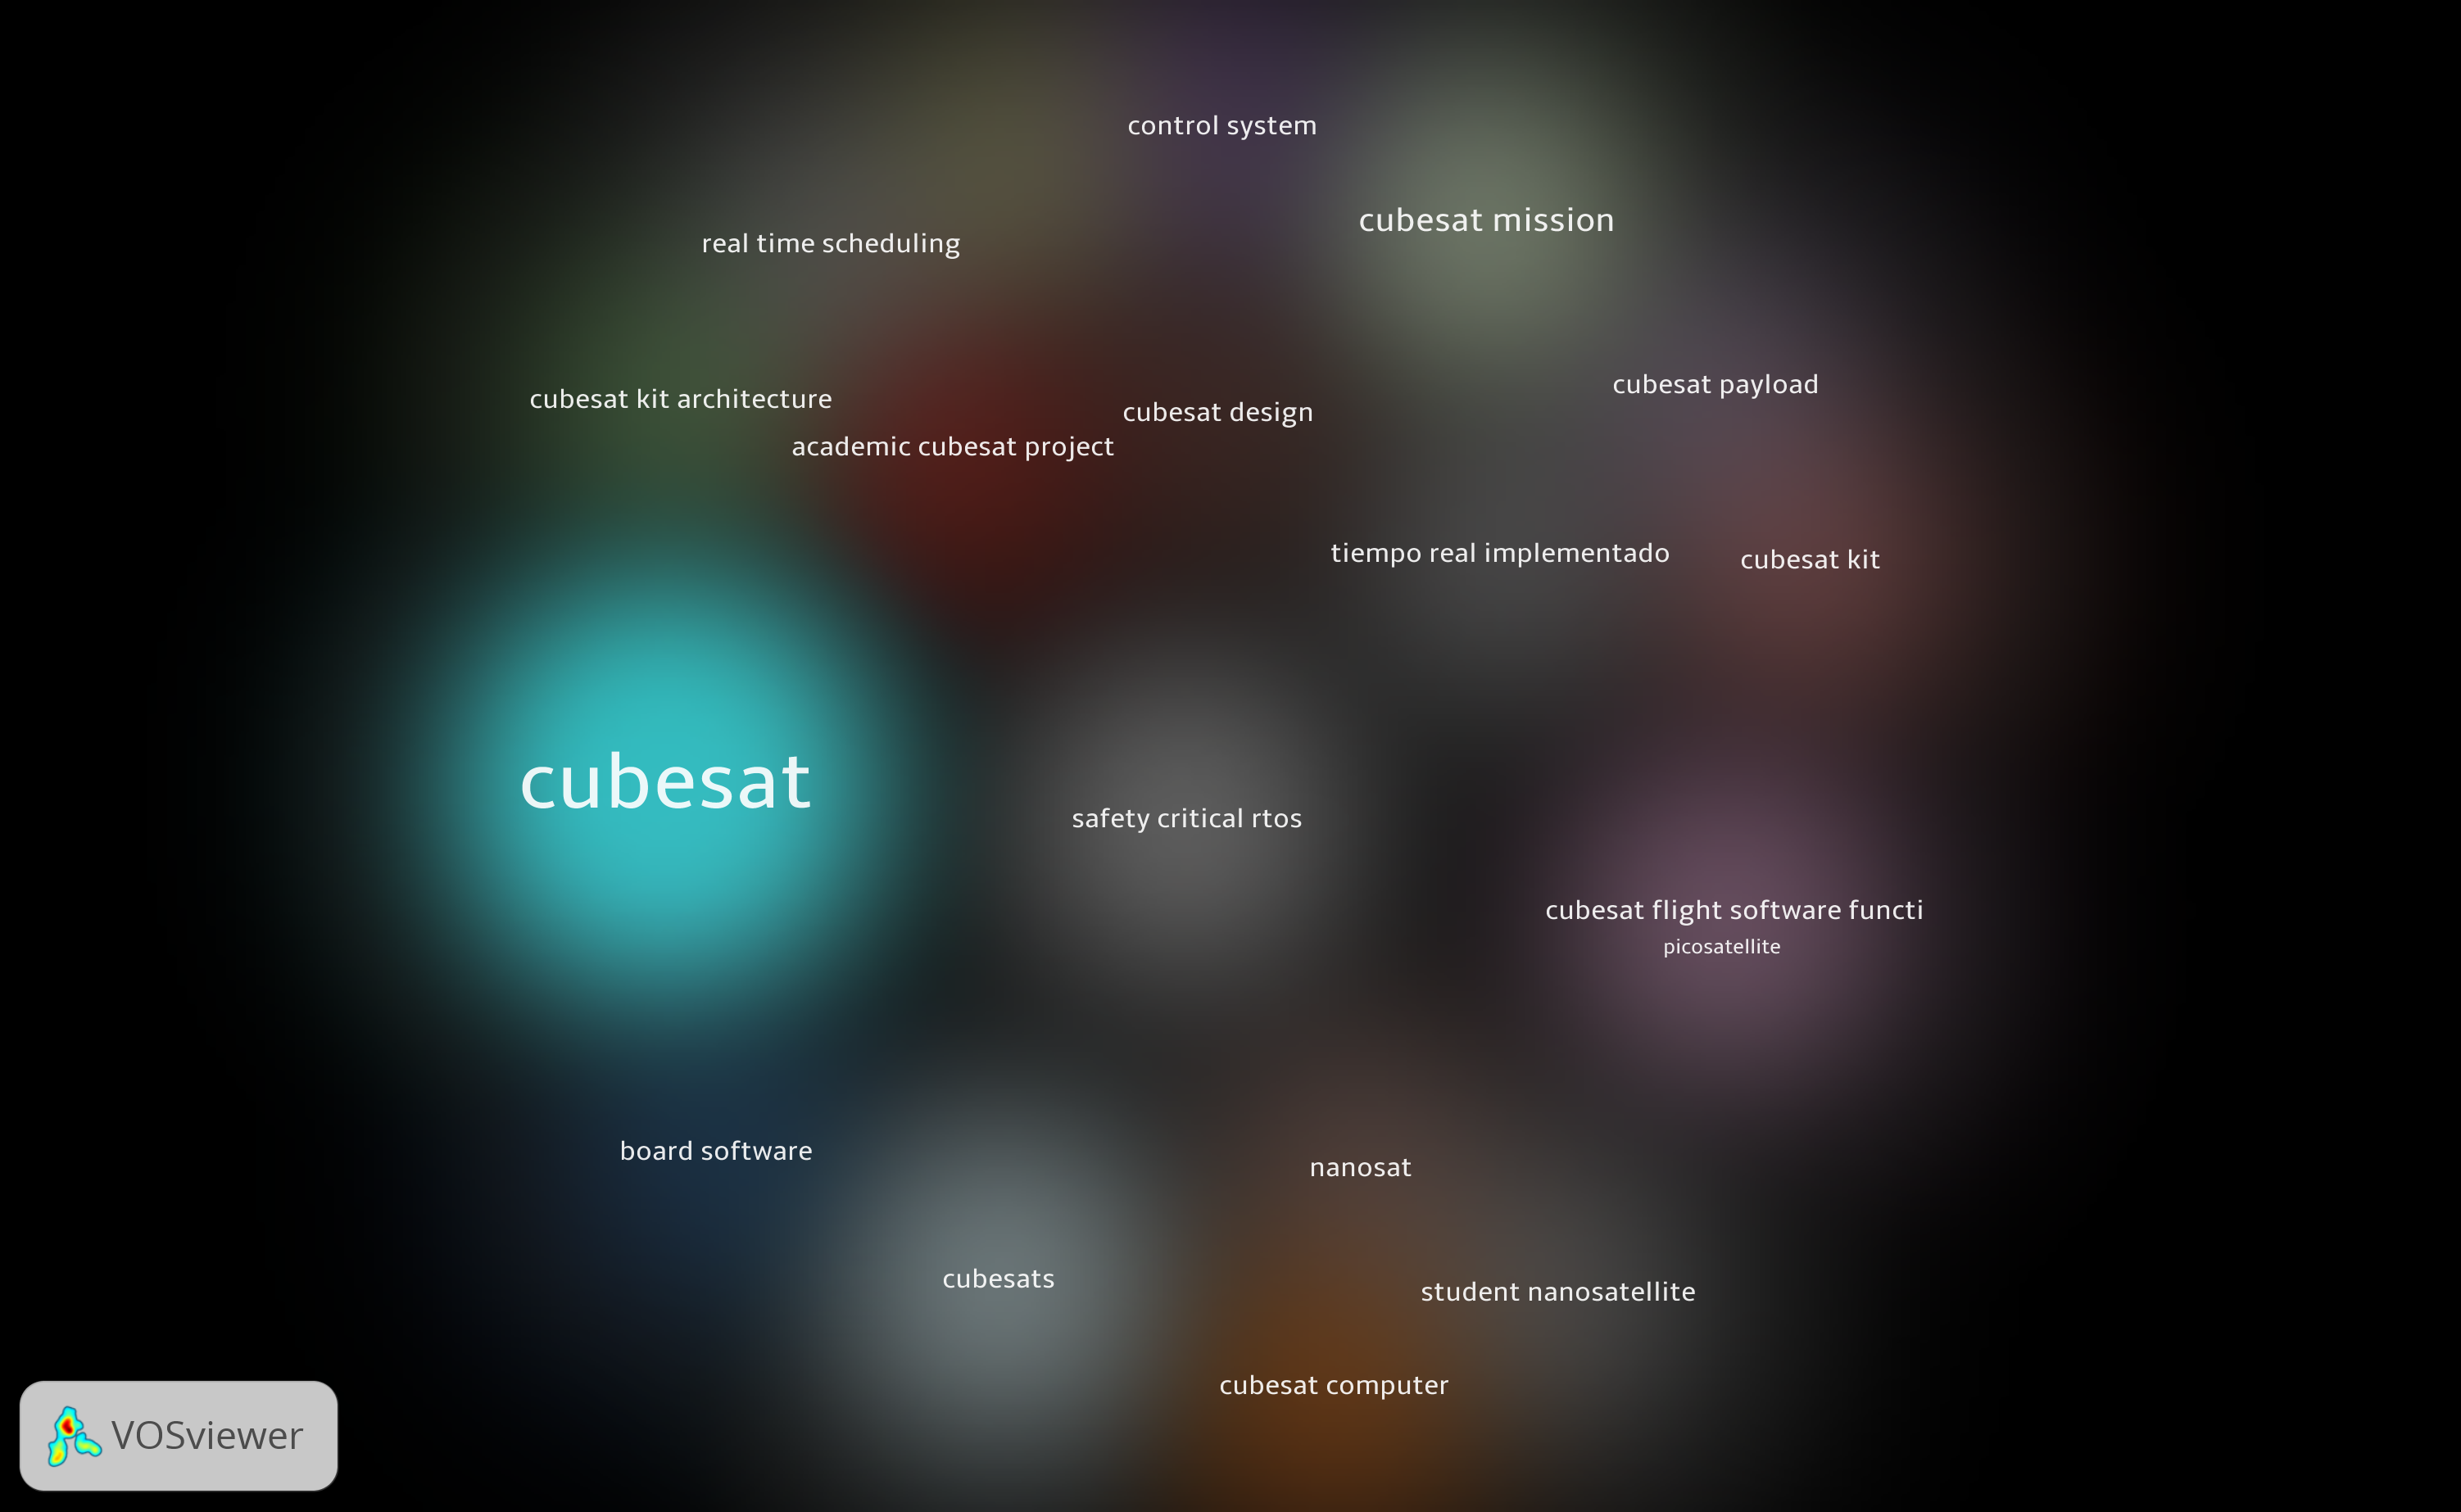
\includegraphics[width=15cm]{imagens/Cubesat_density_central.png}
% 	\caption{Mapa de visualização de densidade sobre o termo "Cubesat SO"}
% 	Fonte: Autor com base no Software VOSViwer.
% 	\label{fig: Cubesat Density Visualization}
% \end{figure}

% Ao redor do termo "cubesat", pode-se observar os termos correlacionado "academic cubesat project", 
% "board software", "safety critical RTOS" e "cubesat kit architeture".Os cluster maiores e com cores mais 
% vivas sinalizam um maior número de citações, a proximidade entre os termos indica correlação entre eles, 
% todos os termos são encontrado sem trabalhos sobre cubesats, uma pesquisa na base de trabalhos Google 
% Acadêmico retornou aproximadamente 16.900 resultados entre os anos de 2012 até 2021. Nota-se, na 
% Figura~\ref{fig: Cubesat Published}, o número de trabalhos publicados por ano tem crescido a elevadas 
% taxas anuais, chegando em 2020 com mais de 2.000 trabalhos publicados e citações contendo os termos 
% "Cubesat SO" em título e resumo.


% \begin{figure}[H]
% 	\centering
% 	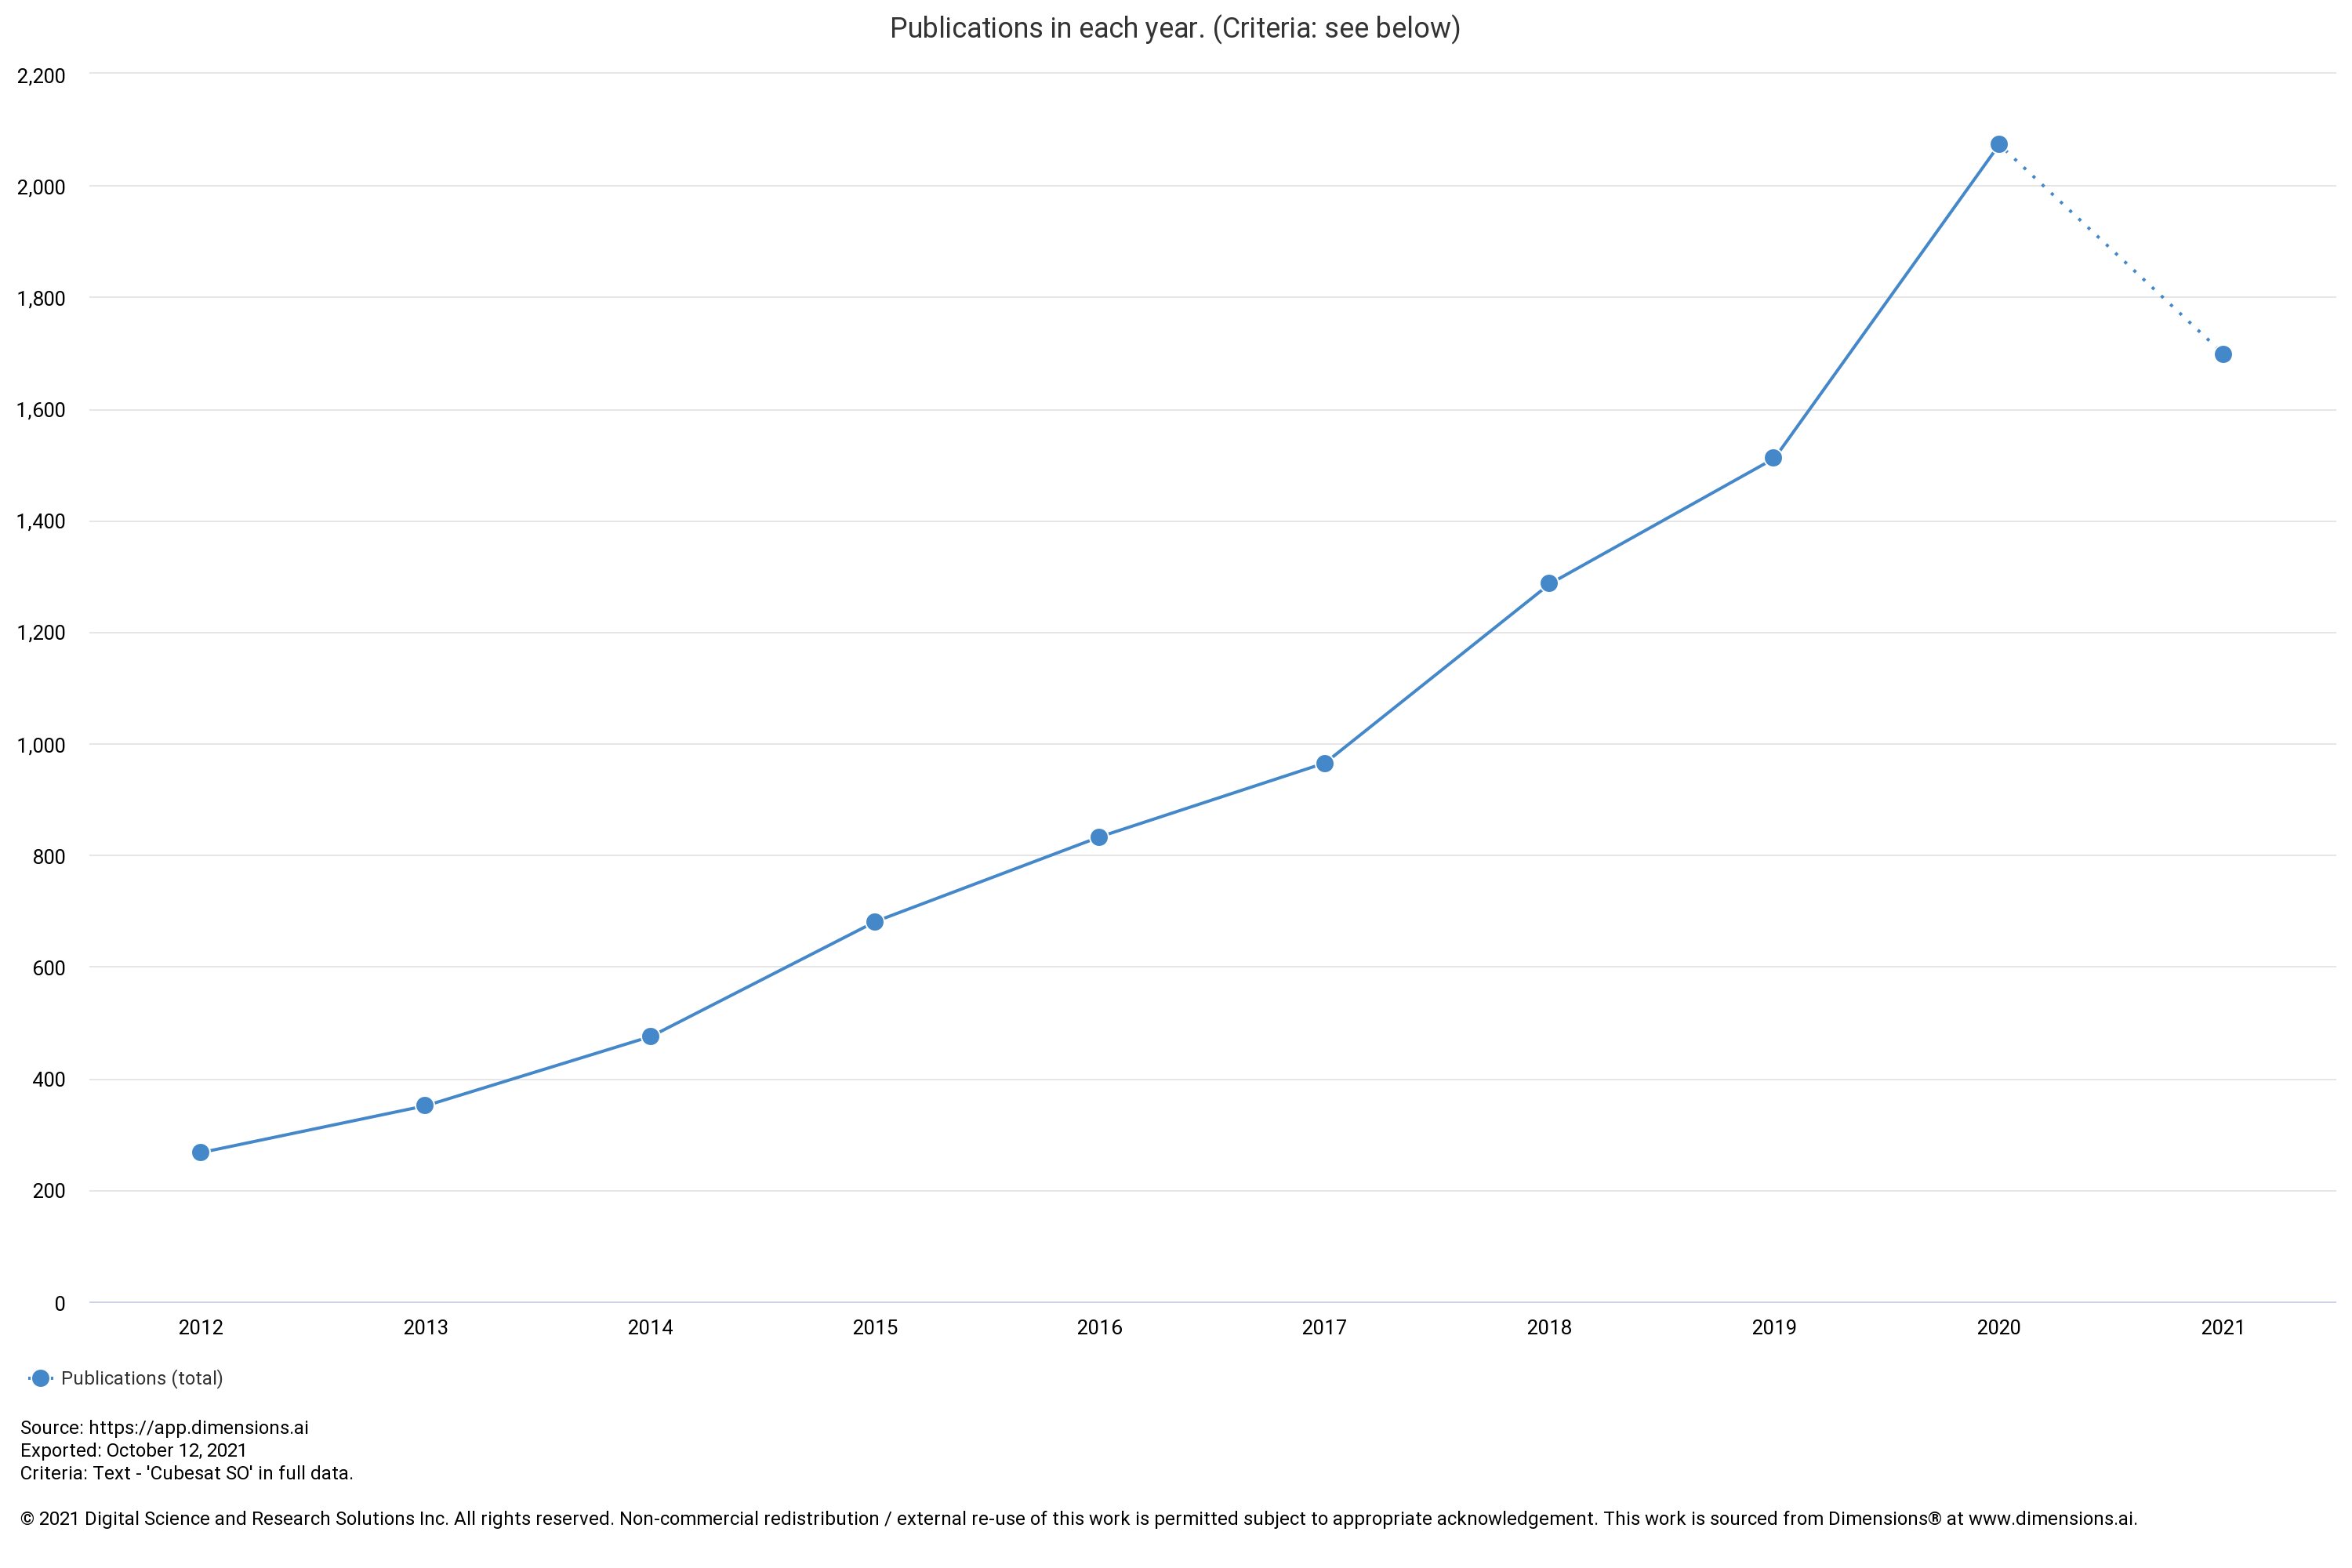
\includegraphics[width=15cm]{imagens/cubesat_publicados.png}
% 	\caption{A visualização mostra o número de publicações publicadas em cada ano de 2012 a 2021.}
% 	Fonte: Autor com base no site "dimensions.ai".
% 	\label{fig: Cubesat Published}
% \end{figure}

% Nota-se que o numero de trabalhos publicados e sempre maior que o ano anterior, reforçando a ideia de 
% que os termos se encontram em destaque no meio acadêmico, com diversos trabalhos sendo correlacionados 
% a iniciativas e nano satélites já concluídos ou em fase final de desenvolvimento. De acordo com \cite{Woellert2011} 
% muitos destes projetos iniciam como spin-offs acadêmicos que terminam como uma atividade comercial.


\subsection{Conclusões sobre a Revisão Bibliométrica realizada}
Percebesse que o estudo na área de tratamento de dados de sensores concentra-se em média uma grande quantidade de trabalhos recentes, com diferentes abordagens de como remover ou reduzir dados ruidosos, apresentando a ideia de que o tema e de interesse atual da comunidade acadêmica mundial. A diversos ramos nos quais tratamento e eliminação de ruídos de sensores podem peregrinar, podendo verificar a ocorrência dos termos em problemas que não necessariamente estão interessados na obtenção do sinal limpo, mas sim na caracterização e coleta dos ruídos na amostra ou que fogem do escopo deste trabalho com a eliminação de ruído, sendo feita através de equipamento físico. 

% Ademais, 
% o levantamento bibliométrico passa a ideia que utilizar Zephyr em um projeto de Cubesat não 
% e uma ideia muito distante, abrindo uma janela de possíveis trabalhos na área que possam 
% trazer grandes contribuições, possibilitando o surgimento deste trabalho.

% Conclusão


% \subsection{Problema da interferência em sensores}

\section{Intervalo de confiança}
Segundo \cite{patino2015intervalos} um IC e a metade da divisão do tamanho do real efeito na população de interesse, essa imprecisão ou diferença entre duas médias é sempre a melhor estimativa dado o tamanho da população atingida. De acordo com \cite{henriques2011dificuldades} o intervalo de confiança é um dos procedimentos gerais de inferência estatística que pode aplicar-se a diversos campos de problemas. Os mais utilizados são estimação de parâmetros desconhecidos de uma população, comparação de distribuições, teste de hipóteses sobre parâmetros populacionais, determinar o tamanho de amostra adequado para realizar uma inferência, e determinar limites de tolerância. Cada um destes campos é muito alargado e variado e incluem a estimação de média, proporção, variâncias, parâmetros de regressão e correlação.  


\section{ Filtro de Kalman}
\cite{tan2005sensoclean} diz que através de uma sequencia de dados observados o filtro de Kalman pode estimar o estado verdadeiro de um sistema dinâmico, o mesmo e utilizado por uma grande parte das aplicações de engenharia que visam sistemas complexos como visão computacional ou radares. O filtro e baseado em probabilidade estatística sendo capaz de suavizar ruídos de sensores eletrônicos visando seu posterior processamento \cite{International_Conference__Zhuang}.

\section{Média Móvel}
De acordo com \cite{santos2021educaccao}, a média móvel é uma técnica que consiste em calcular a média aritmética das observações mais recentes de uma série de dados temporais. Portanto, temos uma estimativa que não leva em consideração a observação mais antiga. Os autores também esclareceram que o nome média móvel foi usado porque a cada período as observações mais antigas são substituídas pelas mais recentes, então uma nova média é calculada.


\section{Média Móvel Ponderada}
Segundo \cite{ribeiro2020analise}, a média móvel ponderada é superior à média móvel simples porque realiza uma mudança de impacto entre os dados de demanda mais antigos e os mais recentes, o que pode revelar algumas tendências. Eles também afirmam que a média móvel simples atribui o mesmo peso a cada componente da série de dados, enquanto a média móvel ponderada permite atribuir um fator de ponderação a cada elemento onde a soma de todos os pesos é igual a um.



% \section{Filtro FIR}

% \section{Filtro IIR}
